\documentclass[a4paper, 12pt, titlepage]{article}
\usepackage[utf8]{inputenc}
\usepackage{geometry}
\usepackage{polski}
\usepackage{graphicx}
\usepackage{float}
\usepackage{etoolbox,refcount}
\usepackage{multicol}
\usepackage{fancyhdr}
\usepackage{listings}
\title{Programowanie robota laboratoryjnego ROB3}
\author{Adrian Jałoszewski, Tomasz Kotowski}
\date{}
\newgeometry{left=2.5cm, right=2.5cm, bottom=2.5cm, top=2.5cm}

\begin{document}
	\maketitle
	\section{Cel ćwiczenia}
		Celem ćwiczenie jest zbudowanie w oprogramowaniu Simulink układu, który pozwoli na sterowanie laboratoryjnym robotem ROB3 oraz napisanie programu sterującego nim.
	\section{Układ w Simulinku}.
		Układ jest regulatorem typu P ograniczonym przez blok nasycenia, podobnie jest z wejściem. Każde wejście ma ustawione inne ograniczenia wynikające z zakresu ruchu danego komponentu. Ze względu na konstrukcję robota należy zastosować sumator, który zamienia wartość zadaną na przeciwną, a nie wartość uzyskaną jako sprzężenie zwrotne -- jest to dalej układ z ujemnym sprzężeniem zwrotnym.
		\begin{figure}[H]
			\centering
			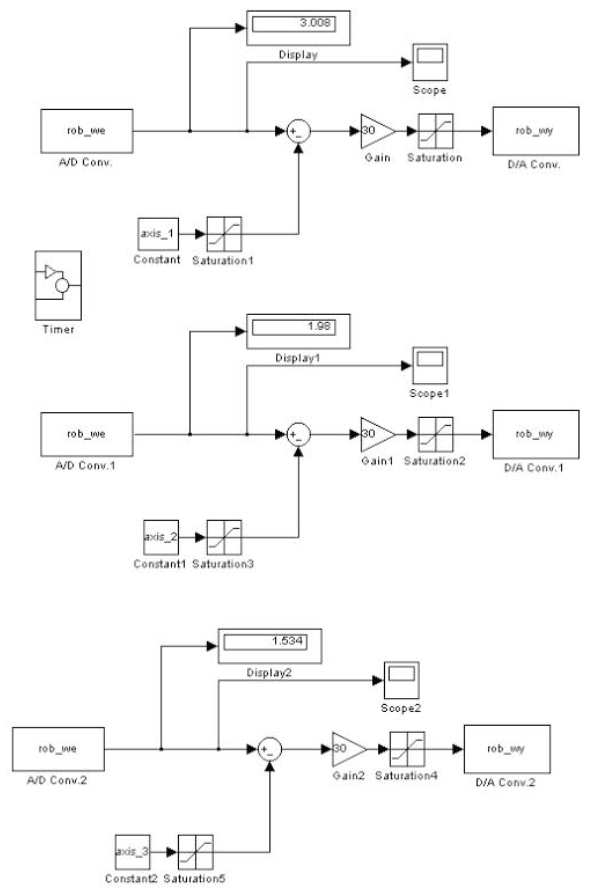
\includegraphics[width=0.65\textwidth]{img/system.png}
			\caption{Układ sterowania}
		\end{figure} \noindent
		Układ sterujący robotem składa się tylko z trzech części, gdyż pozostałe dwie nie działają.
	\section{Program sterujący}
		Program ten miał być napisany w środowisku matlab i miał przedstawiać ruch podobny do rozładowywania palety.
\lstset{language=Matlab} 
\begin{lstlisting}[frame=single, keepspaces=true] 
while (1 == 1)
    rob3axis = [0.5, 2, 2]
    sim('cudo',6)
    rob3axis = [0.5, 2.8, 1.5]
    sim('cudo',3)
    rob3axis = [0.5, 2, 2] 
    sim('cudo',3)
    rob3axis = [3, 2, 2]
    sim('cudo',6)
    rob3axis = [3, 2.8, 1.5]
    sim('cudo',3)
end
\end{lstlisting}
		Kod ten włącza program zrobiony w Simulinku na czas wykonania ruchu, a następnie przechodzi do następnego kroku. Ruch został tak zaprogramowany, aby był płynnie zapętlony. Ze względu na wygodę użytkowania został zastosowany wektor \texttt{rob3axis}, którego wartości pod danym indeksem odpowiadają wartościom zadanym dla robota.
	\section{Wnioski}
		Robot z ćwiczenia realizował ruch przypominający rozładowywanie palety, powracając następnie do położenia początkowego. Czynność była wykonywana wielokrotnie, co w sytuacji obecności działającego chwytaka mogłoby pozwolić na rozładowywanie taśmociągu.
\end{document}